\section{Geschwindigkeit bestimmen}
Um die Sollgeschwindigkeit des Robotinos zu bestimmen, wird das Subsystem Vektorberechnung genutzt. Dieses Subsystem ist wie in Abbildung \ref{fig:Vektorberechnung} dargestellt, aufgebaut. Das Subsystem hat dabei den in Abbildung \ref{fig:AblVektor} gezeigten Ablauf. Dabei ist zu erkennen, dass zuerst die IR Daten erfasst werden und die fahrenden Robotinos erkannt werden. Die IR Datenerfassung wird unter Kapitel \ref{} näher erläutert. Wie die fahrenden Robotinos erkannt werden, wird in Kapitel \ref{} beschrieben. Anhand der IR Daten und der Informationen über die fahrenden Robotinos wird dann der Geschwindigkeitsvektor bestimmt. Die dabei genutzte Funktion wird unter Kapitel \ref{} beschrieben. Anhand des bestimmten Geschwindigkeitsvektors wird dann eine Ausweichrichtung bestimmt, wenn ein anderer Robotino die Route kreuzt. die dazu genutzte Funktion ist in Kapitel \ref{} näher beschrieben. Im nächsten Schritt wird dann das Ausweichmanöver ausgeführt. Die Implementierung des Ausweichmanövers wird in Kapiitel \ref{} beschrieben.

\begin{figure}
	\centering	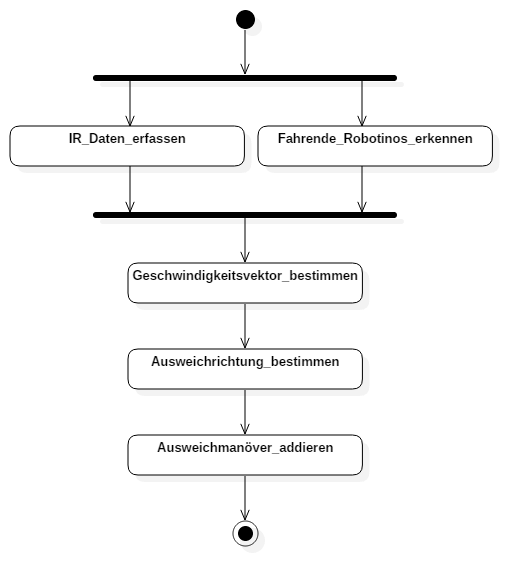
\includegraphics[width=0.5\textwidth]{grafiken/Geschwindigkeit_bestimmen.png}
	\caption{Subsystem Vektorberechnung}
	\label{fig:Vektorberechnung}
\end{figure}

\begin{figure}
	\centering	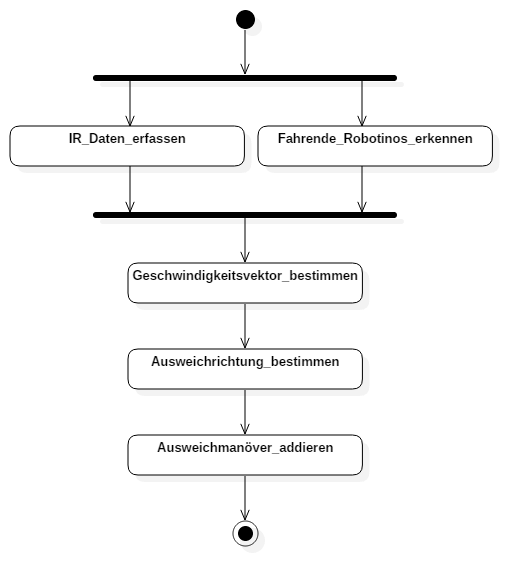
\includegraphics[width=0.5\textwidth]{grafiken/Geschwindigkeit_bestimmen.png}
	\caption{Ablaufplan des Subsystems Vektorberechnung}
	\label{fig:AblVektor}
\end{figure}

\subsection{IR Daten erfassen}
In der IR Daten erfassen Funktion werden zuerst die IR Daten aus den RobotinoDaten gefiltert und auf NaN gesetzt, wenn der gemessene Abstand größer als 150 mm ist. Bei einem Abstand kleiner gleich 150 mm wird die Position der Hindernisse in globalen Koordinaten bestimmt und ausgegeben.

\subsection{Fahrende Robotinos erkennen}
Um zu erkennen ob die anderen Robotinos fahren, werden die Postionen der Robotinos mit den Postionen vor einer Sekunde verglichen. Wenn die Robotinos mehr als 10 mm in der Sekunde zurückgelegt haben, wird der Robotino als fahrend gesetzt.

\subsection{Geschwindigkeitsvektor bestimmen}

\subsection{Ausweichrichtung bestimmen}


\subsection{Ausweichmanöver addieren}
